\documentclass[a4paper, 11pt, normalem]{report}

\usepackage{../../../LaTeX-Templates/Notes}
\usepackage{subfiles}
\usepackage{tensor}
\usetikzlibrary{arrows.meta}
\usetikzlibrary{decorations.markings}
\usetikzlibrary{decorations.pathmorphing}
\tikzset{snake it/.style={decorate,decoration=snake}}

\newcommand\xo{\hat{X}_1}
\newcommand\xt{\hat{X}_2}
\newcommand\hsig{\hat{\sigma}}
\newcommand\hd{\hat{\unl{d}}}
\newcommand\hrho{\hat{\rho}}

\title{General Relativity \vspace{-20pt}}
\author{Richard Bower}
\date{\vspace{-15pt}Epiphany Term 2020}
\rhead{\hyperlink{page.1}{Contents}}

\begin{document}

\maketitle
\tableofcontents
\chapter{}
Just intro stuff

\chapter{Introduction to Tensors}
\begin{itemize}
    \item Notation
    \item Coordinate transforms
    \item Contravariant tensors
    \item Covariant tensors
\end{itemize}

\section{Intro to Tensor Notation}
Consider the cartesian definition for $\vr$:
\begin{align}
    \vr = x\vec{i} + y\vec{j} + \vec{z}.
\end{align}
We have the basis vector $\{\vec{i},\vec{j},\vec{k}\}$ and coordinate values $\{x,y,z\}$.
We can write this in a different form as
\begin{align}
    \vr = x^1\ve_1 + x^2\ve_2 + x^3\ve_3.
\end{align}
Note: $x^2 \neq x*x$.
The 2 is an index, not a power. 
If we want to square something, we will write $(x^1)^2 = x^1x^1$.
We can rewrite the above again as
\begin{align}
    \vr = \sum_{i=1}^3 x^i\ve_i.
\end{align}
We can then simplify this further using the \textbf{Einstein summation convention}:
\begin{align}
    \vr = x^i\ve_i,
\end{align}
i.e. whenever there is a repeated index, we sum over them. 
Different letters will imply different things:
\begin{itemize}
    \item Roman letters $i,j,\dots$ - summing over 3D space
    \item Roman letters $a,b,c,\dots$ - summing over ND space
    \item Roman letters $A,B,\dots$ - summing over 2D space
    \item Greek letters $\alpha,\beta,\mu,\nu,\dots$ - summing over 4D space-time $\{x^0,x^1,x^2,x^3\}$, starting from 0 as time is different slightly, so $\{ct,x^i\}$
\end{itemize}

\section{Coordinate Transformation}
You may be used to 
\begin{align}
    x' = \gamma\left(x-\frac{vct}{c}\right),
\end{align}
where the extra $c$ factor to make time space-like. 
This notation can get confusing so instead we use:
\begin{align}
    x^{\bar{1}} = \gamma\left(x^1-\frac{v}{c}x^0\right),
\end{align}
where the 'bar' indicates new coordinate system. 

For a minute vector difference between points P and Q $d\vr$ in two coordinate systems, we can define $\ve_a$:
\begin{align}
    \vr(P) &= \ve_ax^a & \vr(P) &= \ve_{\bar{b}}x^{\bar{b}} \\
    d\vr &= dx^a\ve_a  \\
    \frac{\p\vr}{\p x^a} &= \ve_a & \frac{\p\vr}{\p x^{\bar{b}}} &= \ve_{\bar{b}}
\end{align}
But what is the relationship between these two coordinate systems?
Start with $x^{\bar{b}}=x^{\bar{b}}(x^a)$, and consider a general function 
\begin{align}
    f &= f(x^1,x^2,x^3) \\
    \Delta f &= \frac{\p f}{\p x^1}\Delta x' + \frac{\p f}{\p x^2}\Delta x^2 + \frac{\p f}{\p x^2}\Delta x^3 = \frac{\p f}{\p x^a}\Delta x^a
\end{align}
How do we get a small change in $x^{\bar{b}}$?
\begin{align}
    \Delta x^{\bar{b}} &= \frac{\p x^{\bar{b}}}{\p x^{a}}\Delta x^{a} \\
    dx^{\bar{b}} &= \frac{\p x^{\bar{b}}}{\p x^a}dx^a \\
    dx^{\bar{a}} &= \frac{\p x^{\bar{a}}}{\p x^b}dx^b
\end{align}
Notice how we can simply just switch round the indices - \textbf{these are all dummy variables and as long as the index notation is consistent, it is completely arbitrary which letter is used,} i.e. the letters themselves mean nothing.

\section{Tensors}
Any quantity which transforms as 
\begin{align}
    A^{\bar{b}} &= \frac{\p x^{\bar{b}}}{\p x^a}A^a
\end{align} 
is a Rank (1,0) or order 1 contravariant tensor.
What about $\ve_a$?
\begin{align}
    \vr &= x^a\ve_a = x^{\bar{b}}\ve_{\bar{b}} \\
    \ve_{\bar{b}} &= \frac{\p\vr}{\p x^{\bar{b}}} = \frac{\p\vr}{\p x^a} \frac{\p x^a}{\p x^{\bar{B}}} = \frac{\p x^a}{\p x^{\bar{b}}}\ve_a
\end{align}
So now we have reversed the position of the indices in Eq (2.15).

How do we define scalars? 
\begin{align}
    \del\phi &= \frac{\p\phi}{\p x^i}\ve_i \\
    \frac{\p\phi}{\p x^{\bar{j}}} &= \frac{\p x^i}{\p x^{\bar{j}}}\frac{\p\phi}{\p x^i}
\end{align}
In general, we have
\begin{align}
    A_{\bar{j}} &= \frac{\p x^i}{\p x^{\bar{j}}}A_i,
\end{align}
which we call a Rank (0,1) or order 1 covariant tensor.

\chapter{}

\section{Higher order tensors}
Consider
\begin{align}
    T^{ab} &= A^aB^b, \\
    T^{\bar{c}\bar{d}} &= A^{\bar{c}}B^{\bar{d}} = \left(\frac{\p x^{\bar{c}}}{\p x^a}A^a\right)\left(\frac{\p x^{\bar{d}}}{\p x^b}B^b\right) = \frac{\p x^{\bar{c}}}{\p x^a}\frac{\p x^{\bar{d}}}{\p x^b}A^a B^b = \frac{\p x^{\bar{c}}}{\p x^a}\frac{\p x^{\bar{d}}}{\p x^b}T^{ab}.
\end{align}
This is the definition of a second order contravariant tensor. 

\section{Tensor Equations}
We can write a basic tensor equation,
\begin{align}
    T^a = k(A^a+B^a),
\end{align}
and wonder how this would look in a transformed coordinate system?
\begin{align}
    T^{\bar{b}} &= \frac{\p x^{\bar{b}}}{\p x^a}T^a = k\left(\frac{\p x^{\bar{b}}}{\p x^a}A^a + \frac{\p x^{\bar{b}}}{\p x^a}B^a\right) \\
                &= k(A^{\bar{b}}+B^{\bar{b}}).
\end{align}
So if a tensor equation is true, it is true in all coordinate systems.

\section{The metric tensor}
What is the metric? \emph{The metric is a measure of space.}
We define the metric tensor, 
\begin{align}
    g_{ab} &= \ve_a\cdot\ve_b = g_{ba},
\end{align}
so it is symmetric.
We can use this when calculating spacetime distances:
\begin{align}
    ds^2 &= \vec{dr}\cdot\vec{dr} = \left(dx^a\ve_a\right)\cdot\left(dx^b\ve_b\right) \\
         &= (\ve_a\cdot\ve_b)dx^a\,dx^b = g_{ab}dx^a\,dx^b.
\end{align}
Is it a tensor?
\begin{align}
    g_{\bar{a}\bar{b}} &= (\ve_{\bar{a}}\cdot\ve_{\bar{b}}) = \left(\frac{\p x^c}{\p x^{\bar{a}}}\ve_c\right)\cdot\left(\frac{\p x^{d}}{\p x^{\bar{b}}}\ve_d\right) \\
                       &= \frac{\p x^c}{\p x^{\bar{a}}}\frac{\p x^d}{\p x^{\bar{b}}}(\ve_c\cdot\ve_d) = \frac{\p x^c}{\p x^{\bar{a}}}\frac{\p x^d}{\p x^{\bar{b}}}g_{cd},
\end{align}
so it transforms as a tensor; a second order covariant tensor. 

\section{Kronecker Delta}
We can write an arbitrary vector as 
\begin{align}
    \vec{A} = A^a\ve_a = A^{\bar{b}}\ve_{\bar{b}} &= \left(\frac{\p x^{\bar{b}}}{\p x^a}A^a\right)\left(\frac{\p x^{d}}{\p x^{\bar{b}}}\ve_d\right) \\
                                                  &= \left(\frac{\p x^{\bar{b}}}{\p x^a}\frac{\p x^{d}}{\p x^{\bar{b}}}\right)A^a\ve_d = \left(\frac{\p x^{d}}{\p x^a}\right)A^a\ve_d \\
                                                  &= \tensor{\delta}{_a^d}A^a\ve_d = A^d\ve_d = A^a\ve_a
\end{align}

\chapter{}

\chapter{}

\chapter{}
Asbolute Derivative:
\begin{align}
    \frac{D\lambda^a}{ds} &= \frac{d\lambda^a}{ds} + \tensor{\Gamma}{^a_{bc}}\lambda^b\frac{dx^c}{ds}
\end{align}
Covariant Derivative:
\begin{align}
    \tensor{\lambda}{^a_{;c}} &= \frac{\p\lambda^a}{\p x^c}+\tensor{\Gamma}{^a_{bc}}\lambda^b
\end{align}
Christoffel Symbols:
\begin{align}
    \tensor{\Gamma}{^c_{ab}}\ve_c &= \frac{\p\ve_a}{\p x^b},\quad \tensor{\Gamma}{^c_{ab}} = \tensor{\Gamma}{^c_{ba}}
\end{align}
Other stuff:
\begin{align}
    \frac{\p g_{ab}}{\p x^c} &= \tensor{\Gamma}{^d_{ac}}g_{bd} + \tensor{\Gamma}{^d_{bc}}g_{ad}\\
    \frac{\p g_{bc}}{\p x^a} &= \tensor{\Gamma}{^d_{ba}}g_{cd} + \tensor{\Gamma}{^d_{ca}}g_{bd}\\
    \frac{\p g_{ca}}{\p x^b} &= \tensor{\Gamma}{^d_{cd}}g_{ad} + \tensor{\Gamma}{^d_{ab}}g_{cd}\\
    2\tensor{\Gamma}{^d_{ac}}g_{bd} &= \frac{\p g_{ab}}{\p x^c} + \frac{\p g_{bc}}{\p x^a} - \frac{\p g_{ca}}{\p x^b} \\
    \tensor{\Gamma}{^f_{ac}} &= \frac12 g^{fb}\left(\frac{\p g_{bc}}{\p x^a} - \frac{\p g_{ca}}{\p x^b} + \frac{\p g_{ab}}{\p x^c}\right) \\
                             &= \frac12 g^{fb}\left(\p_a g_{bc} - \p_b g_{ca} + \p_c g_{ab}\right)
\end{align}
We multiplied lefthandside of (6.7) by $\tensor{\delta}{^f_d}$.

\begin{example}[2D flat space]
    $x^A = \{x,y\}$:
    \begin{align}
        g_{AB} &= \begin{pmatrix} 1 & 0 \\ 0 & 1 \end{pmatrix} = \text{diag}(1,1) \\
        \tensor{\Gamma}{^A_{BC}} &= 0 
    \end{align}
    So we don't have to deal with these in Cartesian coordinates. What about polar coordinates? $x^A = \{r,\theta\}$:
    \begin{align}
        ds^2 &= dr^2 + r^2\,d\theta^2 \\
        g_{AB} &= \text{diag}(1,r^2) \\
        \tensor{\Gamma}{^A_{BC}} \neq 0 
    \end{align}
    So we can still get non-zero Christoffel symbols even for flat space, but it is still "boring" really. 
\end{example}

Let's consider something more interesting, i.e. curved. 
For 3D space, we have
\begin{align}
    ds^2 &= dr^2 + r^2\,d\theta^2 + r^2\sin^2\theta\,d\phi^2 
\end{align}
But we want to use just the surface of a sphere, so fixed $r=a$:
\begin{align}
    ds^2 &= a^2\,d\theta^2 + a^2\sin^2\theta\,d\phi^2 = g_{AB}dx^A\,dx^B \\
    g_{AB} &= \text{diag}(a^2,a^2\sin^2\theta)
\end{align}
We have $g_{AB}$, but we want $g^{AB}$. Recall
\begin{align}
    g^{AB}g_{BC} &= \tensor{\delta}{^A_C}.
\end{align}
So we have a set of 4 simultaneous equations:
\begin{align}
    g^{A1}g_{1C} + g^{A2}g_{2C} &= \tensor{\delta}{^A_C}.
\end{align}
For diagonal $g_{AB}$ \textbf{ONLY}:
\begin{align}
    g^{AB}g_{BA} &= g^{AA}g_{AA} = 1 \implies g^{AA} = \frac{1}{g_{AA}} \\
    g^{AB} &= \text{diag}\left(\frac{1}{a^2},\frac{1}{a^2\sin^2\theta}\right)
\end{align}
So now we want to calculate
\begin{align}
    \tensor{\Gamma}{^\theta_{\theta\theta}} &= \frac12 g^{\theta B} \left(\p_\theta g_{B\theta} - \p_B g_{\theta\theta} + \p_{\theta} g_{\theta B}\right), \quad g^{\theta B} = 0, B\neq\theta \\
                                            &= \frac12 \frac{1}{a^2}\left(\p_{\theta} g_{\theta\theta} - \p_\theta g_{\theta\theta} + \p_\theta g_{\theta\theta}\right) =  0 \\
    \tensor{\Gamma}{^\theta_{\phi\theta}} = \tensor{\Gamma}{^\theta_{\theta\phi}} &= \frac12 g^{\theta B}\left(\p_\theta g_{B\phi} - \p_B g_{\phi\theta} + \p_\phi g_{\theta B}\right) \\
                                          &= \frac12 g^{\theta\theta}\left(\p_\theta g_{\theta\phi} - \p_\theta g_{\phi\theta} + \p_\phi g_{\theta\theta}\right) = 0 \\
    \tensor{\Gamma}{^\theta_{\phi\phi}} &= -\sin\theta\cos\theta \\
    \tensor{\Gamma}{^\phi_{\theta\phi}} &= \cot\theta
\end{align}
The rest of the Christoffel symbols for this example are 0 (there are $2^3=8$ in total?).

\section{Geodesic Equations}
The velocity is a tensor,
\begin{align}
    \vec{v} &= v^\alpha\ve_{\alpha} = \frac{\p x^\alpha}{\p\tau}\ve_\alpha
\end{align}
If there's no force, then there's no change in the velocity vector doesn't change, but its components might change. 
No force means the absolute derivative of the components: 
\begin{align}
    \frac{Dv^\alpha}{d\tau} &= 0
\end{align}
By an affine parameter, we mean a linear function of path length $u=A+Bs$, such as the proper time $\tau$.
\begin{align}
    \frac{dv^\alpha}{d\tau} + \tensor{\Gamma}{^\alpha_{\beta\gamma}}v^\beta\frac{dx^\gamma}{d\tau} &= 0 \\
    \frac{d^2x^\alpha}{d\tau^2} + \tensor{\Gamma}{^\alpha_{\beta\gamma}}\frac{dx^\beta}{d\tau}\frac{dx^\gamma}{d\tau} &= 0 \\
    \ddot{x}^\alpha + \tensor{\Gamma}{^\alpha_{\beta\gamma}}\dot{x}^\beta\dot{x}^\gamma &= 0
\end{align}
Let's guess and make a solution for the sphere, $s=a\theta$, so we are just going around the circumference of the sphere at constant $\phi$.
For $\theta$:
\begin{align}
    \frac{d^2\theta}{ds^2} + \tensor{\Gamma}{^\theta_{BC}}\frac{dx^B}{ds}\frac{dx^c}{ds} = 0 + \tensor{\Gamma}{^\theta_{\phi\phi}}\frac{d\phi}{ds}\frac{d\phi}{ds} = 0
\end{align}
We get a big tick and a gold star!
For $\phi$:
\begin{align}
    \frac{d^2\phi}{ds^2} + \tensor{\Gamma}{^\phi_{BC}}\frac{dx^B}{ds}\frac{dx^C}{ds} = 0 + \tensor{\Gamma}{^\phi_{\theta\phi}}\frac{d\theta}{ds}\frac{d\phi}{ds} + \tensor{\Gamma}{^\phi_{\phi\theta}}\frac{d\phi}{ds}\frac{d\theta}{ds} = 0 
\end{align}
So it's a geodesic path! Yayyyyyy!


\chapter{}

\chapter{}
Last lecture:
\begin{itemize}
    \item Euler-Lagrange equations 
    \item 'easier' way to find $\tensor{\Gamma}{^a_{bc}}$
    \item how to find Geodesic paths
\end{itemize}

This lecture:
\begin{itemize}
    \item more tensor derivatives
\end{itemize}
Recall absolute derivative again:
        \begin{align}
            \frac{D\lambda^a}{ds} &= \frac{d\lambda^a}{ds} + \tensor{\Gamma}{^a_{bc}}\lambda^b\frac{dx^c}{ds}.
        \end{align}
The first term above is the total change, and then the second is to ``subtract off the change due to the coordinate system".
So for parallel transport, this means there is no physical change, i.e.
\begin{align}
    \frac{D\lambda^a}{ds} = 0.
\end{align}
The absolute derivative obeys normal rules for derivatives.
\begin{itemize}
    \item Linear operator -
        \begin{align}
            \frac{D}{ds}\left(\lambda^a+ k\mu^a\right) = \frac{D\lambda^a}{ds} + k\frac{D\mu^a}{ds}.
        \end{align}
    \item The (Leibniz) chain rule -
        \begin{align}
            \frac{D}{ds}\left(\lambda^a\mu^b\right) = \mu^b\frac{D\lambda^a}{ds} + \lambda^a\frac{D\mu^b}{ds}.
        \end{align}
\end{itemize}
What is the absolute derivative of a scalar, $\phi$?
$\phi$ does not depend on the coordinates as tensors do, so it would just be the normal derivative, i.e. 
\begin{align}
    \frac{D\phi}{ds} = \frac{d\phi}{ds}.
\end{align}
We have defined the absolute derivative of a contravariant tensor, but now what about a covariant tensor $\mu_a$?
We can write a scalar as $\phi=\lambda^a\mu_a$, so we can write
\begin{align}
    \frac{D\phi}{ds} &= \frac{D}{ds}(\lambda^a\mu_a) = \mu_a\frac{D\lambda^a}{ds}+\lambda^a\frac{D\mu_a}{ds}, \\
    \frac{d\phi}{ds} &= \mu_a\left(\frac{d\lambda^a}{ds} + \tensor{\Gamma}{^a_{bc}}\lambda^b\frac{dx^c}{ds}\right) + \lambda^a\frac{D\mu_a}{ds}, \\
    \lambda^a\frac{d\mu_a}{ds} &= \mu_a\tensor{\Gamma}{^a_{bc}}\lambda^b\frac{dx^c}{ds} + \lambda^a\frac{D\mu_a}{ds}, \\
                               &= \mu_b\tensor{\Gamma}{^b_{ac}}\lambda^a\frac{dx^c}{ds} + \lambda^a\frac{D\mu_a}{ds},
\end{align}
where $\lambda^a$ is any tensor, so if this is true, it must be true for any $\lambda^a$.
We can then `cancel' $\lambda^a$ through unity, as the remaining equation must also be true:
\begin{align}
    \frac{d\mu_a}{ds} &= \tensor{\Gamma}{_{ac}^b}\mu_b\frac{dx^c}{ds} + \frac{D\mu_a}{ds}, \\
    \frac{D\mu_a}{ds} &= \frac{d\mu_a}{ds} - \tensor{\Gamma}{_{ac}^b}\mu_b\frac{dx^c}{ds}.
\end{align}
This is the absolute derivative of a convariant tensor. 

What is the absolute derivative of a rank (1,1) tensor $\tensor{\tau}{^a_b}=\lambda^a\mu_b$?
\begin{align}
    \frac{D\tensor{\tau}{^a_b}}{ds} = \frac{D(\lambda^a\mu_b}{ds} &= \mu_b\frac{D\lambda^a}{ds} + \lambda^a\frac{D\mu_b}{ds}, \\
                                                                  &= \mu_b\left[\frac{d\lambda^a}{ds}+\tensor{\Gamma}{^a_{dc}}\lambda^d\frac{dx^c}{ds}\right] + \lambda^a\left[\frac{d\mu_b}{ds}-\tensor{\Gamma}{_{bc}^d}\mu_d\frac{dx^c}{ds}\right],\\
    \frac{D\tensor{\tau}{^a_b}}{ds} &= \frac{d}{ds}(\lambda^a\mu_b) + \tensor{\Gamma}{^a_{dc}}\tensor{\tau}{^d_b}\frac{dx^c}{ds} - \tensor{\Gamma}{_{bc}^d}\tensor{\tau}{_d^a}\frac{dx^c}{ds}.
\end{align}
This is the absolute derivative for a rank (1,1) tensor.

What about the covariant derivative?
It is defined as:
\begin{align}
    \tensor{\lambda}{^a_{;c}} &= \frac{\p\lambda^a}{\p x^c} + \tensor{\Gamma}{^a_{bc}}\lambda^b \\
    \frac{D\lambda^a}{ds} &= \tensor{\lambda}{^a_{;c}}\frac{dx^c}{ds} \\
                          &= \frac{\p\lambda^a}{\p x^c}\frac{dx^c}{ds} + \tensor{\Gamma}{^a_{bc}}\lambda^b\frac{dx^c}{ds} = \frac{d\lambda^a}{ds} + \dots.
\end{align}
All the rules still apply, so we can write out the covariant derivative for a scalar, a covariant, and a higher order tensor:
\begin{align}
    \phi_{;c} &= \frac{\p\phi}{\p x^c}, \\
    \mu_{a;c} &= \frac{\p\mu+a}{\p x^c}-\tensor{\Gamma}{_{ac}^b}\mu_b, \\
    \lambda_{ab;c} &= \frac{\p\lambda_{ab}}{\p x^c} - \tensor{\Gamma}{_{ac}^d}\lambda_{db}-\tensor{\Gamma}{_{bc}^d}\lambda_{ad}.
\end{align}
We can also consider the metric:
\begin{align}
    g_{ab;c} &= ? \\
    \frac{\p g_{ab}}{\p x^c} &= \frac{\p}{\p x^c} (\ve_a\cdot\ve_b), \\
                             &= \frac{\p\ve_a}{\p x^c}\cdot\ve_b + \ve_a\cdot\frac{\p\ve_b}{\p x^c},\\
                             &= \left(\tensor{\Gamma}{_{ac}^d}\ve_d\right)\cdot\ve_b + \ve_a\cdot\left(\tensor{\Gamma}{_{bc}^d}\ve_d\right), \\
                             &= \tensor{\Gamma}{_{ac}^d}g_{db} + \tensor{\Gamma}{_{bc}^d}g_{ad}, \\
    g_{ab;c} &= \frac{\p g_{ab}}{\p x^c} - \tensor{\Gamma}{_{ac}^d}g_{db} - \tensor{\Gamma}{_{bc}^d}g_{ad} = 0,
\end{align}
where we used the previous definitions of the covariant derivative to find this definition. 
Why is this important?
The metric allows us to switch coordinate systems as
\begin{align}
    R_a &= g_{ab}R^b.
\end{align}
Now suppose we want to find the covariant derivative:
\begin{align}
    R_{a;c} &= \cancel{g_{ab;c}R^b} + g_{ab}\tensor{R}{^b_{;c}} \\
            &= g_{ab}\tensor{R}{^b_{;c}}.
\end{align}

\chapter{}
\section{The Riemann Curvature Tensor}
\begin{itemize}
    \item how do we know if space is curved?
    \item second derivatives of the metric
    \item `space-sing' around a loop
    \item convergence of geodesic paths
\end{itemize}
The Riemann curvature tensor tells us \emph{how much the direction of a vector changes as it goes round a loop}, or the \emph{tidal forces of gravity}.
\begin{align}
    \tensor{\left(\tensor{\lambda}{^a_{;b}}\right)}{_{;c}} &= \frac{\p\tensor{\lambda}{^a_{;b}}}{\p x^c} + \tensor{\Gamma}{^a}{_{ec}}\tensor{\lambda}{^e_{;b}} - \tensor{\Gamma}{_{bc}^f}\tensor{\lambda}{_{;f}^a} \\
                                                         &= \frac{\p}{\p x^c}\left(\frac{\p\lambda^a}{\p x^b} + \tensor{\Gamma}{^a_{bd}}\lambda^d\right) + \cdots \\
    \tensor{\lambda}{^a_{;b;c}} &= \frac{\p^2\lambda^a}{\p x^c \p x^b} + \tensor{\Gamma}{^d_{bd}}\frac{\p\lambda^d}{\p x^c} + \lambda^d\frac{\p\tensor{\Gamma}{^a_{bd}}}{\p x^c} + \tensor{\Gamma}{^a_{ec}}\tensor{\lambda}{^a_{;b}}-\tensor{\Gamma}{_{bc}^f}\tensor{\lambda}{^a_{;f}} 
\end{align}
In flat space, the Christoffel symbols go to zero, so we can sway $;b$ and $;c$ indices, but \textbf{not in curved space.}
\begin{align}
    \tensor{\lambda}{^a_{;c;b}} &= \frac{\p^2\lambda^a}{\p x^b\p x^c} + \tensor{\Gamma}{^a_{cd}}\frac{\p\lambda^d}{\p x^b} + \lambda^d\frac{\p\tensor{\Gamma}{^a_{cd}}}{\p x^b} + \tensor{\Gamma}{^a_{eb}}\tensor{\lambda}{^e_{;c}} - \tensor{\Gamma}{_{cb}^f}\tensor{\lambda}{^a_{;f}} \\
    \tensor{\lambda}{^a_{;c;b}}-\tensor{\lambda}{^a_{;b;c}} &= \left(\tensor{\Gamma}{^a_{cd}}\frac{\p\lambda^d}{\p x^b} - \tensor{\Gamma}{^a_{bd}}\frac{\p\lambda^d}{\p x^c}\right) + \lambda^d\left(\frac{\p\tensor{\Gamma}{_{cd}^a}}{\p x^b} - \frac{\p\tensor{\Gamma}{_{bd}^a}}{\p x^c}\right) + \left(\tensor{\Gamma}{^a_{eb}}\tensor{\lambda}{^e_{;c}}-\tensor{\Gamma}{^a_{ec}}\tensor{\Gamma}{^e_{;b}}\right) \\
                                                            &= \tensor{\Gamma}{^a_{cd}}\left(\frac{\p\lambda^a}{\p x^b}-\tensor{\lambda}{^d_{;b}}\right) + \tensor{\Gamma}{^a_{bd}}\left(\tensor{\lambda}{^d_{;c}}-\frac{\p\lambda^d}{\p x^c}\right) + \lambda^d\left(\frac{\p\tensor{\Gamma}{^a_{cd}}}{\p x^b} - \frac{\p\tensor{\Gamma}{^a_{bd}}}{\p x^c}\right) \\
                                                            &= \left(\tensor{\Gamma}{^a_{be}}\tensor{\Gamma}{^e_{cd}} - \tensor{\Gamma}{^a_{ce}}\tensor{\Gamma}{^e_{bd}} + \frac{\p\tensor{\Gamma}{^a_{cd}}}{\p x^b} - \frac{\p\tensor{\Gamma}{^a_{bd}}}{\p x^c}\right)\lambda^d = \tensor{R}{^a_{dbc}}\lambda^d
\end{align}
We have arrived at the Riemann curvature tensor.
Consider:
\textit{doodle diagram}
\begin{align}
    \lambda^a(B^1) &= \lambda^a(A) + \tensor{\lambda}{^a_{;b}}\delta x^b + \tensor{\lambda}{^a_{;c}}\delta y^c + \tensor{\lambda}{^a_{;b;c}}\delta x^b\delta y^c \\
    \lambda^a(B^2) &= \lambda^a(A) + \tensor{\lambda}{^a_{;c}}\delta y^c + \tensor{\lambda}{^a_{;b}}\delta x^b + \tensor{\lambda}{^a_{;c;b}}\delta y^c\delta x^b \\
    \Delta\lambda^a &= \lambda^a(B^2)-\lambda^a(B^1) = \left(\tensor{\lambda}{^a_{;c;b}}-\tensor{\lambda}{^a_{;b;c}}\right)\delta x^b\delta y^c \\
                    &= \tensor{R}{^a_{dbc}}\lambda^a\cdot\text{ area of loop}
\end{align}
In flat space, any two lines have a separation that increases linearly with distance $s$, e.g. $\p_s^2=0$.
But in curved space, our two lines can converge or diverge as they travel from initial parallel conditions. 
Consider two lines $x^a(s)$ and $\tilde{x}^a(s)$ with a separation $\zeta^a=\tilde{x}^a - x^a$.
We can write our geodesic equation for this as
\begin{align}
    \frac{d^2x^a}{ds^2} &+ \tensor{\Gamma}{^a_{bc}}\frac{dx^b}{ds} \frac{dx^c}{ds} = 0 \\
    \frac{d^2\tilde{x}^a}{ds^2} &+ \tensor{\tilde{\Gamma}}{^a_{bc}}\frac{d\tilde{x}^b}{ds}\frac{d\tilde{x}^c}{ds} = 0 \\
    \ddot{\zeta}^a &+ \tensor{\Gamma}{^a_{bc}}\dot{x}^b\dot{\zeta}^c + \tensor{\Gamma}{^a_{bc}}\dot{\zeta}^b\dot{x}^c + \frac{\p\tensor{\Gamma}{^a_{bc}}}{\p x^d} \zeta^d\dot{x}^b\dot{x}^c = 0  \\
    \frac{D^2\zeta^a}{ds^2} &= \frac{D}{ds}\left(\dot{\zeta}^a + \tensor{\Gamma}{^a_{bc}}\zeta^b\dot{x}^c\right) \\
                            &= \ddot{\zeta}^a + \tensor{\Gamma}{^a_{bc}}\zeta^b\dot{x}^c + \frac{d}{ds}\left(\tensor{\Gamma}{^a_{bc}}\zeta^b\dot{x}^c\right)+\tensor{\Gamma}{^a_{ef}}\left(\tensor{\Gamma}{^e_{bc}}\zeta^b\dot{x}^c\right)\dot{x}^f
\end{align}

\chapter{}
\emph{Things are about to get a little more physics!} - Richard Bower. \\
In this lecture:
\begin{itemize}
    \item Geodesic convergence.
    \item Symmetry of the Riemann tensor, 
        \begin{align}
            \tensor{R}{^a_{dbc}} &= \tensor{\Gamma}{^a_{bc}}\tensor{\Gamma}{^e_{cd}} - \tensor{\Gamma}{^a_{ce}}\tensor{\Gamma}{^e_{bd}} + \p_b\tensor{\Gamma}{^a_{cd}}-\p_c\tensor{\Gamma}{^a_{bd}}.
        \end{align}
    \item We will look towards Einstein's equations by combining our knowledge of movement in curved space with gravity. 
    \item We will do this through the stress-energy tensor, $T^{\mu\nu}$. (Not as simple as it could be, R has four indices, this has two, but we'll get to that.)
    \item This will lead towards to conservation laws in GR.
\end{itemize}
At the end of last lecture, we considered divergent lines with a spatially-dependent separation $\zeta$:
\begin{align}
    \ddot{x}^a + \tensor{\Gamma}{^a_{bc}}\dot{x}^b\dot{x}^c &= 0 \\
    \ddot{\tilde{x}}^a + \tensor{\tilde{\Gamma}}{^a_{bc}}\dot{x}^b\dot{x}^c &= 0 \\
    \ddot{\zeta} + \tensor{\Gamma}{^a_{bc}}\dot{x}^b\dot{\zeta}^c + \tensor{\Gamma}{^a_{bc}}\dot{\zeta}^b\dot{x}^c + \frac{\p\tensor{\Gamma}{^a_{bc}}}{\p x^d}\zeta^d\dot{x}^b\dot{x}^c &= 0.
\end{align}
We want to find the Tensor equation from this! 
\begin{align}
    \frac{D^2\zeta^a}{ds^2} &= \ddot{\zeta}^a + \tensor{\Gamma}{^a_{bc}}\dot{\zeta}^b\dot{x}^c + \frac{d}{ds}\left(\tensor{\Gamma}{^a_{bc}}\zeta^b\dot{x}^c\right) + \tensor{\Gamma}{^a_{ef}}\left(\tensor{\Gamma}{^a_{bc}}\zeta^b\dot{x}^c\right)\dot{x}^f.\\
    \frac{d}{ds}\left(\tensor{\Gamma}{^a_{bc}}\zeta^b\dot{x}^c\right) &= \tensor{\Gamma}{^a_{be}}\zeta^b\ddot{x}^e + \tensor{\Gamma}{^a_{bc}}\dot{\zeta}^b\dot{x}^c + \zeta^b\dot{x}^c\left(\frac{\p\tensor{\Gamma}{^a_{bc}}}{\p x^d}\dot{x}^d\right).
\end{align}
So we expanded out the derivative to get rid of something we didn't want, and now combine for the final result (as well as using the definition of a geodesic path, $\ddot{x}^e=-\tensor{\Gamma}{^e_{cd}}\dot{x}^c\dot{x}^d$, in Eq. (10.5)):
\begin{align}
    \frac{D^s\zeta^a}{ds^2} &+ \left(\tensor{\Gamma}{^a_{be}}\tensor{\Gamma}{^e_{cd}}-\tensor{\Gamma}{^a_{ce}}\tensor{\Gamma}{^e_{bd}}+\p_b\tensor{\Gamma}{^a_{cd}}-\p_c\tensor{\Gamma}{^a_{bd}}\right)\zeta^b\dot{x}^c\dot{x}^d = 0.
\end{align}
This looks very confused as it is, but we can simplify by now defining the Riemann tensor:
\begin{align}
    \frac{D^2\zeta}{ds^2} &+ \tensor{R}{^a_{dbc}}\zeta^b\dot{x}^c\dot{x}^d = 0,\\
    \tensor{R}{^a_{dbc}} &= \tensor{\Gamma}{^a_{bc}}\tensor{\Gamma}{^e_{cd}} - \tensor{\Gamma}{^a_{ce}}\tensor{\Gamma}{^e_{bd}} + \p_b\tensor{\Gamma}{^a_{cd}}-\p_c\tensor{\Gamma}{^a_{bd}}.
\end{align}
From this definition, we can quickly infer the symmetry relation
\begin{align}
    \tensor{R}{^a_{dcb}} &= -\tensor{R}{^a_{dbc}}.
\end{align}

\section{Symmetries of the Riemann tensor}
In 4D space-time, the Riemann tensor contains $4\times4\times4\times4 = 256$ numbers. 
This isn't very fun unless you are a computer, says Richard.
However, using the symmetry of the Riemann tensor, there are only 20 indepedent elements, which can be a lot easier. 
How do we demonstrate this though?
We can use mathematical tricks for tensors, whereby if we prove something in one coordinate system, it must be true in all coordinate systems.

\subsection{Local Geodesic Coordinates}
Local geodesic coordinates describe a flat space at a local point in curved space.
We know, therefore, that we can write the metric at this point as
\begin{align}
    g_{\alpha\beta} &= \begin{pmatrix} 1 & 0 & 0 & 0 \\ 0 & -1 & 0 & 0 \\ 0 & 0 & -1 & 0 \\ 0 & 0 & 0 & -1 \end{pmatrix},
\end{align}
which is known as the \textbf{Minkowski metric} for flat space. 
This is familiar from special relativity, where it represents the usual Minkowski product,
\begin{align}
    ds^2 &= c^2\,d\tau^2 = c\,dt^2 - dx^2 - dy^2 - dz^2.
\end{align}
So the Christoffel symbol at this local point is
\begin{align}
    \tensor{\Gamma}{^\alpha_{\beta\gamma}} &= 0,
\end{align} 
where we have only chosen a point to set this locally to zero. 
However, the derivatives will not be zero, as if we move away from this local point, space will become curved again:
\begin{align}
    \frac{\p\tensor{\Gamma}{^\alpha_{\beta\gamma}}}{\p x^\delta} &= 0.
\end{align}
Now this will allow us to simplify the Riemann tensor from its definition in Eq. (10.9), where it can now be written as
\begin{align}
    \tensor{R}{^a_{dbc}} &= \p_b\tensor{\Gamma}{^a_{cd}} - \p_c\tensor{\Gamma}{^a_{bd}}.
\end{align}
What about the symmmetry relations of this simplified Riemann tensor?
\begin{align}
    \tensor{R}{^a_{cdb}} &= \p_d\tensor{\Gamma}{^a_{bc}} - \p_b\tensor{\Gamma}{^a_{dc}}, \\
    \tensor{R}{^a_{bcd}} &= \p_c\tensor{\Gamma}{^a_{db}} - \p_d\tensor{\Gamma}{^a_{cb}}. 
\end{align}
What about the sum of these three tensors?
Due to the symmetry of the Christoffel symbols' lower indicies, we can see that there will be lots of cancellations in this sum, leading to
\begin{align}
    \tensor{R}{^a_{dbc}} + \tensor{R}{^a_{cdb}} + \tensor{R}{^a_{bcd}} &= 0,
\end{align}
which is known as the cyclic relation of the Riemann tensor.
The Riemann tensor can also be written in its covariant form:
\begin{align}
    \tensor{R}{_{abcd}} &= g_{ae}\tensor{R}{^e_{bcd}}.
\end{align}
In its covariant form, we can also go through similar steps to above to prove other symmetry relations, including:
\begin{align}
    R_{abcd} &= -R_{bacd}, & R_{abcd} &= -R_{abdc}, & R_{abcd} &= R_{cdab}.
\end{align}
From these relations, we see that repeated indices can lead to zero, such as
\begin{align}
    R_{aacd} = -R_{aacd} &\implies R_{aacd} = 0, \\
    R_{abcc} = -R_{abcc} &\implies R_{abcc} = 0.
\end{align}
This allows us to neglect many of the 256 numbers as they will be zero, reducing the total of free elements of the Riemann tensor to 20.

\section{How can we relate this to gravity?}
Let's consider Eq. (10.4) for low speeds, i.e. non-relativistic. 
\begin{align}
    \zeta^\alpha = \begin{pmatrix} 0, & 0, & y, & 0 \end{pmatrix},
\end{align}
i.e. we have a simple separation in the y-direction between the two geodesic paths. 
We would then get something like
\begin{align}
    \frac{D^y}{ds^2} &= -\tensor{R}{^2_{020}}yc^2,
\end{align}
where we only consider the indices relating to $y$ and time. 
This should look somewhat familiar. 
What would we have written for this in Newtonian physics, if we have these two objects both moving towards a large mass $M$ with a separation $y$ and a distance from the massive object $r$?
\begin{align}
    \frac{d^2y}{dt^2} &= -\frac{GM}{r^2}\cdot\frac{y}{r}.
\end{align}
Important note: the massive object is the Sun or a molecular cloud or something, according to Richard.
\textbf{A black hole wouldn't be happy, you wouldn't be able to tell.}

Using $ds=c\,dt$:
\begin{align}
    c^2\frac{d^2y}{ds^2} &= -\frac{GM}{r^3}y,\\
    -\frac{GM}{r^3} &= -\tensor{R}{^2_{020}}.
\end{align}
So we now have an equivalence of curved space and Newtonian gravitational force. 
We can see that the Newtonian expression in Eq. (10.27) is the energy density of space, if mass and energy can be equivalent.
This is what lead Einstein to his famous equations. 

\section{What is energy?}
Energy is special relativity was defined in
\begin{align}
    E &= \gamma m_0c^2,
\end{align}
where we can now relate the mass and energy of objects.
We also have a number density, $n_0$, for the number of particles ``in a box" or in the universe or whatever you're considering. 
Recall from special relativity the four-velocity of a system:
\begin{align}
    u^\alpha &= \frac{dx^\alpha}{dt} = \gamma\begin{pmatrix} c, & -\frac{dx^i}{dt}\end{pmatrix}.
\end{align}
There is also the four-momentum of the system:
\begin{align}
    p^\alpha &= m_0u^\alpha = \gamma m_0\begin{pmatrix} c, & -\frac{dx^i}{dt} \end{pmatrix}.
\end{align}
The number per unit volume is $\gamma n_0$.
We also have a flux through the surface,
\begin{align}
    N^\rho &= n_0u^\rho.
\end{align}
Using all this, we can write down an expression for the energy-momentum density:
\begin{align}
    T^{\mu\nu} &= N^\mu p^\nu = n_0u^\mu m_0u^\nu = \rho_0 u^\mu u^\nu.
\end{align}
In the rest frame, these two velocities will each be $c$, so the $T^{00}$ term will get us back to Eq. (10.28) as $\rho_0 c^2$.

\chapter{}

\chapter{}

\chapter{}

\chapter{}

\chapter{}

\chapter{Time and Black Holes}
\begin{itemize}
    \item Last lecture - orbits around black holes
    \item This lecture - time depends on \unl{where you are} and \unl{how you move}; falling into a black hole
\end{itemize}

\section{The Schwarzchild Metric}
Defined as 
\begin{align}
    ds^2 &= c^2d\tau^2 = c^2\left(1-\frac{2m}{r}\right)dt^2 - \left(1-\frac{2m}{r}\right)^{-1}dr^2 - r^2d\phi^2.
\end{align}
An observer experiences the proper time, $\tau$, whereas $t$ is the time coordinate.
\textit{doodle}
For the coordinate time seen from the distant observer,
\begin{align}
    t_{orb} &= 2\pi\left(\frac{r^3}{mc^2}\right)^{1/2}.
\end{align}
What does $S_0$ measure?
\begin{align}
    d\tau_0 &= \left(1-\frac{3m}{r}\right)^{1/2}dt,\\
    \tau_{orb} &= \left(1-\frac{3m}{r}\right)^{1/2}t_{orb}
\end{align}
which tells us that there are no orbits possible with $r<3m$.
For the rocket $S_1$, we arrange such that $d\phi=0,dr=0$, i.e. the rocket is being held stationary.
We then get from the metric
\begin{align}
    c^2d\tau_1^2 &= c^2\left(1-\frac{2m}{r_1}\right)dt^2, \\
    \tau_{hov} &= \left(1-\frac{2m}{r_1}\right)^{1/2}t_{orb},\\
    \tau_{orb} &\neq \tau_{hov}.
\end{align}
Consider the example where $r=r=6m$.
We will get 
\begin{align}
    \tau_{orb} &= \left(\frac12\right)^{1/2}t_{orb}, & \tau_{hov} &= \left(\frac23\right)^{1/2}t_{orb}, & \frac{\tau_{orb}}{\tau_{hov}} &= \frac{\sqrt{3}}{2} = 0.86.
\end{align}
So $S_1$ perceives themselves as older than $S_0$.

\section{Radial Geodesics}
Similar to before, but simpler form:
\begin{align}
    c^2d\tau^2 &= c^2\left(1-\frac{2m}{r}\right)dt^2 - \left(1-\frac{2m}{r}\right)^{-1}dr^2. \\
    \left(1-\frac{2m}{r}\right)\dot{t} &= E,
\end{align}
where we have solved the Euler-Lagrange equation in $t$, and $\dot{t}$ is $\frac{dt}{d\tau}$, and $E$ is a constant.
Dividing by $d\tau^2$, we rewrite as
\begin{align}
    c^2 &= c^2\left(1-\frac{2m}{r}\right)\dot{t}^2 - \left(1-\frac{2m}{r}\right)^{-1}\dot{r}^2, \\
    c^2 &= c^2\left(1-\frac{2m}{r}\right)^{-1}E^2 - \left(1-\frac{2m}{r}\right)^{-1}\dot{r}^2, \\
    \dot{r}^2 &- c^2E^2 + c^2\left(1-\frac{2m}{r}\right) = 0.
\end{align}
We need to find constant, so we use the condition $\dot{r}=0$ at $r\gg2m$:
\begin{align}
    -c^2E^2 &+ c^2 = 0, \quad E = 1, \\
    \dot{r}^2 &- c^2 + c^2\left(1-\frac{2m}{r}\right) = 0, \\
    \dot{r}^2 &= \frac{2mc^2}{r} \implies \dot{r}^2 = -c\sqrt{\frac{2m}{r}},
\end{align}
where we have chosen the negative solution for when we are approaching the black hole. 
This looks pretty Newtonian, but remember that $\dot{r}=\frac{dr}{d\tau}$, where $\tau$ is the proper time. 
So this would be the speed measured by the falling observer.

How long does it take to reach $r=0$?
We can work out the proper time as observed by the person falling into the black hole, as
\begin{align}
    \tau &= \int_{r_1}^{r_2} \frac{d\tau}{dr}dr = \int_{r_1}^{r_2} \frac{1}{\dot{r}}dr = \frac{1}{c\sqrt{2m}}\int_{r_2}^{r_1} r^{1/2}\,dr = \frac{2}{3c\sqrt{2m}}\left(r_1^{3/2} - r_2^{3/2}\right).
\end{align}
We have a perfectly finite $\tau$ for $r_2=0$, e.g. $r_1=10m$, $r_2=0$ results in $\tau=14.9\frac{m}{c}$.

If we consider the perspective of the person a long distance away, then 
\begin{align}
    \frac{dr}{dt} &= \frac{dr}{d\tau}\frac{d\tau}{dt} = -c\sqrt{\frac{2m}{r}}\left(1-\frac{2m}{r}\right).
\end{align}
At $r=2m,\frac{dr}{dt}\to0$.
From a distance, we will observe them fall in to the black hole, but slow down and ``stop" at the event horizon; the person falling into the black hole will feel themselves falling in faster and faster. 
We have a gravitational redshift, 
\begin{align}
    \frac{\lambda_R}{\lambda_E} &= \sqrt{\frac{1-\frac{2m}{r_2}}{1-\frac{2m}{r_E}}},
\end{align}
so the wavelength received $\lambda_R\to\infty$.
It isn't quite that we see it come to rest, but rather its signal slowly fades out and gets weaker and weaker until we don't observe anything.

Now let's look at dropping off at some general radius. 
Drop the satellite at $r=r_0,\dot{r}=0$ at $r=0$.
\begin{align}
    E & \sqrt{1-\frac{2m}{r_0}},\\
    \dot{r}^2 &= c^2\left[\left(1-\frac{2m}{r_0}\right)-\left(1-\frac{2m}{r}\right)\right] \\
              &= c^2\left(\frac{2m}{r} - \frac{2m}{r_0}\right), \\
    \dot{t} &= \left(1-\frac{2m}{r}\right)^{-1}\sqrt{1-\frac{2m}{r_0}},\\
    \frac{dr}{dt} = \frac{\dot{r}}{\dot{t}} &= c\sqrt{\frac{2m}{r}-\frac{2m}{r_0}}\frac{\left(1-\frac{2m}{r}\right)}{\sqrt{1-\frac{2m}{r_0}}}.
\end{align}
We can also consider what happens for the hovering observer:
\begin{align}
    dR_h &= \sqrt{1-\frac{2m}{r}}\,dr,\quad  d\tau_h = \sqrt{1-\frac{2m}{r}}\,dr, \\
    \frac{dR_h}{d\tau_h} &= \frac{dR_h}{dr}\frac{dr}{dt}\frac{dt}{d\tau_h} = \left(1-\frac{2m}{r}\right)^{-1}\frac{dr}{dt} = -c\sqrt{\frac{\frac{2m}{r}-\frac{2m}{r_0}}{1-\frac{2m}{r_0}}}.
\end{align}
If we hover at $r_0=2m,r=2m$, then $\frac{dR_h}{d\tau_h}=c$. 
This is quite strange. 
Let's check:
\begin{align}
    \frac{d^2R_h}{d\tau_h^2} &= \frac{d}{d\tau_h}\left(\frac{dR_h}{d\tau_h}\right) = -\frac{mc^2}{r^2}\frac{\sqrt{1-\frac{2m}{r}}}{\left(1-\frac{2m}{r_0}\right)}.
\end{align}
If $r\to\infty\implies$ Newtonian physics is back. 
If $r_0\to2m$, then $\frac{d^2R_h}{d\tau_h}\to\infty$.
However, hovering at $r=2m$ requires an infinitely powerful rocket - you can't hover at $r\leq2m$, i.e. 
\begin{figure}[H]
    \centering
    
\includegraphics[scale=0.7]{gg.jpg}
\end{figure}

\chapter{}
Falling into a black hole!
We have better ways of describing space-time. 
For radial paths, we have the metric and the E-L equations:
\begin{align}
    c^2d\tau^2 &= c^2\left(1-\frac{2m}{r}\right)\,dt^2 - \left(1-\frac{2m}{r}\right)^{-1}dr^2 \\
    \dot{t} &= \left(1-\frac{2m}{r}\right)^{-1},\quad \dot{r} = \sqrt{\frac{2m}{r}}
\end{align}
$\dot{t}$ is dropped as $\to\infty$.
We will define a new time coordinate and it can rewritten as
\begin{align}
    c\,dT &= cd\tau = c\left(1-\frac{2m}{r}\right)\,dt, \\
    c\,dT &= c\,dt - \frac{2mc}{r}\,dt,\\
    dt &= \frac{\dot{t}}{\dot{r}} = \left(\frac{-1}{1-\frac{2m}{r}}\right)\sqrt{\frac{2m}{r}}\frac{1}{c}dr, \\
    c\,dT &= c,dt + \sqrt{\frac{2m}{r}}\left(1-\frac{2m}{r}\right)^{-1}\,dr, \\
    c^2d\tau^2 &= \left(1-\frac{2m}{r}\right)\left[c\,dT - \sqrt{\frac{2m}{r}}\left(1-\frac{2m}{r}\right)\,dr\right]^2 - \left(1-\frac{2m}{r}\right)^{-1}\,dr^2, \\
    c^2d\tau^2 &= \left(1-\frac{2m}{r}\right)c^2dT^2 - 2\sqrt{\frac{2m}{r}}c\,dT\,dr - dr^2.
\end{align}
We now have a rewritten metric in terms of a time coordinate of someone falling into a black hole. 
$\tau$ is the proper time on the radial path, $T$ is the proper time of the falling observer. 
So we can now solve in the falling observer's perspective rather than the orbiting observer.

What do we need to consider causally around the centre of the Black Hole?
\begin{figure}[H]
    \centering
    \begin{tikzpicture}
        \draw[-Latex] (0,0) -- (4,0) node[anchor=north] {r};
        \draw[-Latex] (0,0) -- (0,3) node[anchor=east] {$ct$};
        \draw[dashed] (0,1.5) -- (4,1.5);
        \fill (3,1.5) circle (3pt);
        \draw (2.7,0.8) -- (3.3,0.8) -- (2.7,2.2) -- (3.3,2.2) -- cycle;
%        \fill (3,1.5) circle (3pt);
%        \draw (2.6,0.8) -- (3.4,0.8) -- (2.6,2.2) -- (3.4,2.2) -- cycle;
%        \fill (2.5,1.5) circle (3pt);
%        \draw (2.6,0.8) -- (3.4,0.8) -- (2.6,2.2) -- (3.4,2.2) -- cycle;
%        \fill (3,1.5) circle (3pt);
%        \draw (2.6,0.8) -- (3.4,0.8) -- (2.6,2.2) -- (3.4,2.2) -- cycle;
    \end{tikzpicture}
\end{figure}
\emph{finish doodle}
For photons, we have the null geodesic:
\begin{align}
    0 &= c^2\left(1-\frac{2m}{r}\right)\,dt^2 - \left(1-\frac{2m}{r}\right)^{-1}\,dr^2 \\
    c^2dt^2 &= \left(1-\frac{2m}{r}\right)^{-2}dr^2 \\
    c\frac{dt}{dr} &= \pm \left(1-\frac{2m}{r}\right)^{-1}
\end{align}
This breaks down as we approach the Schwarzchild radius.
We need to think of a new coordinate system to describe the universe. 

\section{Eddington-Finkelstein Coordinates}
If we define 
\begin{align}
    dr_{*} &= \left(1-\frac{2m}{r}\right)^{-1}\,dr \implies \frac{dt}{dr_{*}} = \pm c
\end{align}
photons will not allows propagate at 45 degrees in space-time diagrams, to the expense of our radial coordinate.
If we integrate this,
\begin{align}
    r_{*} &= r + 2m\log\bigg|\frac{r}{2m}-1\bigg|, \\
    ct &= \pm r_{*} + v.
\end{align}
So we have a choice of two equations for defining our time variable, but we must choose one. 
They chose the inward-going light rays for
\begin{align}
    v &= r_{*} + ct, \\
    \frac{dv}{dr} &= \frac{dr_{*}}{dr} + c\frac{dt}{dr}, \\
    dv &= \left(1-\frac{2m}{r}\right)^{-1}dr + cdt.
\end{align}
Again, we can substitute this in to the metric, and find a new form:
\begin{align}
    d\tau^2 &= \left(1-\frac{2m}{r}\right)\,dv^2 - 2\,dv\,dr.
\end{align}
When $v$ is constant and we set $d\tau=0$ we have the path taken by a photon. 
We can solve for the photon paths:
\begin{enumerate}
    \item Inwards propagating, so $dv = 0$ 
    \item 
        \begin{align}
            \frac{dv}{dr} &= \frac{2}{\left(1-\frac{2m}{r}\right)}
        \end{align}
\end{enumerate}
Plotting this, for
\begin{figure}[H]
    \centering
    \begin{tikzpicture}
        \draw[-Latex] (0,0) -- (4,0) node[anchor=north] {r};
        \draw[-Latex] (0,0) -- (0,3) node[anchor=east] {$v$};
    \end{tikzpicture}
\end{figure}
\emph{finish doodle}
Light ray which is always horizontal - would want both at 45 degrees.
Light cone tips over at $r=2m$.
Transform variables again for
\begin{align}
    ct_{*} &= v-r \\
    \frac{cdt_{*}}{dr} &= -1 \\
    \frac{cdt_{*}}{dt} &= \frac{\left(1+\frac{2m}{r}\right)}{\left(1-\frac{2m}{r}\right)}
\end{align}
\emph{another doodle}
\begin{figure}[H]
    \centering
    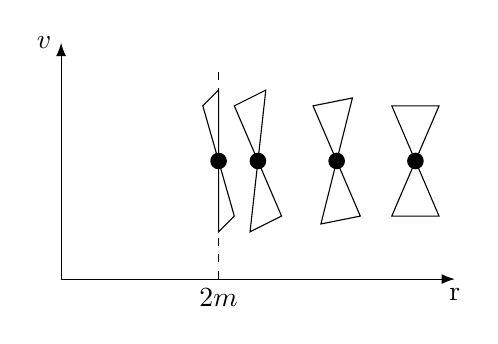
\begin{tikzpicture}
        \draw[-Latex] (-1,0) -- (4,0) node[anchor=north] {r};
        \draw[-Latex] (-1,0) -- (-1,3) node[anchor=east] {$v$};
        \fill (3.5,1.5) circle (3pt);
        \draw (3.2,0.8) -- (3.8,0.8) -- (3.2,2.2) -- (3.8,2.2) -- cycle;
        \fill (2.5,1.5) circle (3pt);
        \draw (2.3,0.7) -- (2.8,0.8) -- (2.2,2.2) -- (2.7,2.3) -- cycle;
        \fill (1.5,1.5) circle (3pt);
        \draw (1.4,0.6) -- (1.8,0.8) -- (1.2,2.2) -- (1.6,2.4) -- cycle;
        \draw[dashed] (1,0) node[anchor=north] {$2m$} -- (1,2.7);
        \fill (1,1.5) circle (3pt);
        \draw (1,0.6) -- (1.2,0.8) -- (0.8,2.2) -- (1,2.4) -- cycle;
    \end{tikzpicture}
\end{figure}
At large $r$, it always travels at 45 degrees. 
The cones of influence are tipping over as the outward ray moves less and less, until we reach $r=2m$ and the outward propagating ray becomes purely time-like and cannot propagate outwards.
Once we're inside this radius, both light rays are then tipping over and both move towards the centre of the black hole as our term in Eq. (17.22) goes negative for both.
The zones of influence are aimed inwards to the Black Hole.

\chapter{}
\section{Initial Overview}
\begin{itemize}
    \item We had the \textbf{Principle of Equivalence} - all bodies feel the same gravity
    \item Mass $\implies$ curved space $\implies$ curved paths \emph{Yoda meme here}
    \item In Special Relativity, we had
        \begin{align}
            \begin{split}
                c^2d\tau^2 &= c^2dt^2 - dx^2 - dy^2 - dz^2 \\
                           &= \eta_{\alpha\beta}dx^\alpha dx^\beta,
            \end{split}
        \end{align}
        where we can express this using the Minkowski metric $\eta_{\alpha\beta}$.
    \item Einstein realised we can express this in a more general metric in General Relativity:
        \begin{align}
            c^2d\tau^2 &= g_{\alpha\beta}dx^\alpha dx^\beta,\quad g_{\alpha_\beta} = (\ve_{\alpha}\cdot\ve_{\beta}).
        \end{align}
    \item $\frac{\p\lambda^\beta}{\p x^\alpha} \implies \tensor{\lambda}{^\beta_{j\alpha}}$.
\end{itemize}

\section{Tensor Maths Toolkit}
We now need to figure out ways to represent everything in tensors.
This follows from defining contra- variant and covariant tensors respectively:
\begin{align}
    A^{\bar{b}} &= \frac{\p x^{\bar{b}}}{\p x^a}A^a, & A_{\bar{b}} &= \frac{\p x^a}{\p x^{\bar{b}}}A_a.
\end{align}
We can convert between these two forms using 
\begin{align}
    \lambda_b &= g_{ab}\lambda^a,
\end{align}
where we need to remember we are using the Einstein Summation Convention over repeated indices.

\section{Geodesic paths and curved space}
When you move a tensor around in curved space, you get changes due to how the coordinate space changes. 
To accomodate for this, we introduce the Total Derivative:
\begin{align}
    \frac{D\lambda^a}{ds} &= \frac{d\lambda^a}{ds} + \tensor{\Gamma}{^a_{bc}}\lambda^b\frac{dx^c}{ds} = \tensor{\lambda}{^a_{;c}}\frac{dx^c}{ds}, \\
    \tensor{\lambda}{^a_{;c}} &= \frac{\p\lambda^a}{\p x^c} + \tensor{\Gamma}{^a_{bc}}\lambda^b, \\
    \tensor{\Gamma}{^f_{bc}} &= \frac12 g^{bf}\left(\p_a g_{bc} - \p_b g_{ca} + \p_c g_{ab}\right).
\end{align}
We then introduce the concept of \emph{parallel transport}, which led us to geodesic paths:
\begin{align}
    \ddot{x}^a + \tensor{\Gamma}{^a_{bc}}\dot{x}^b\dot{x}^c = 0.
\end{align}
For working in equations of motion, we turn to the Euler-Lagrange equations. 
So we express our Lagrangian and then write the E-L equation:
\begin{align}
    \La &= \frac12 g_{\alpha\beta}\dot{x}^\alpha\dot{x}^\beta, & \frac{d}{d\tau}\left(\frac{\p\La}{\p\dot{x}^a}\right) - \frac{\p\La}{\p x^\alpha} &= 0.
\end{align}
The definition of geodesic paths and Euler-Lagrange equation are equivalent, although generally we will find the E-L equation easier to work with. 
This is all well and good, but then we realised that the Riemann curvature tensor $\tensor{R}{^a_{dbc}}$ was like the `second derivative' and can tell us a lot about space.
But we can't equate this with our other tensors yet. 

\section{Eintein's Equations}
We want to describe how mass and the shape of space are related. 
This is derived in the \textbf{Stress-Energy Tensor}:
\begin{align}
    T^{\mu\nu} &= \left(\rho_0+\frac{p}{c^2}\right)u^\mu u^\nu - Pg^{\mu\nu},
\end{align}
so the `00' element describes energy, and the other elements describe momentum. 
In the last term above, we subtract by pressure to get the right form. 
All of physics then can be written as
\begin{align}
    \tensor{T}{^{\mu\nu}_{;\mu}} &= 0.
\end{align}
To help equate different quantities, we introduce the Ricci tensor, which is a \emph{compressed} form of the Riemann tensor:
\begin{align}
    R_{\mu\nu} &= \tensor{R}{^\alpha_{\mu\nu\alpha}}.
\end{align}
We can then compress the Ricci tensor by performing its trace, yielding the \textbf{Curvature Scalar}:
\begin{align}
    \mathcal{R} &= \tensor{R}{^\alpha_\alpha}.
\end{align}
Einstein then used all this to define his `guess' as a way of writing down a relation between the curvature of space and the stress-energy:
\begin{align}
    \left(R^{\mu\nu}-\frac12 g^{\mu\nu}\mathcal{R}\right) &= \kappa T^{\mu\nu}.
\end{align}
Turns out this wasn't quite right - there is also a small \emph{cosmological constant} that needs to be added, which is famous for being Einstein's big blunder. 
The metric is then useful to be redefined once we have reached this point, so we now introduce the Schwarzschild Metric, defining $m=\frac{GM}{c^2}$:
\begin{align}
    c^2d\tau^2 &= c^2\left(1-\frac{2m}{r}\right)\,dt^2 - \left(1-\frac{2m}{r}\right)^{-1}\,dr^2 - r^2d\theta^2 - r^2\sin^2\theta\,d\phi^2.
\end{align}
The rest of the lecture series was pretty much focused on how we solve this metric in different regimes.
\begin{itemize}
    \item Particles in weak gravity - here, we seemed to recover essentially Newtonian physics, with slight corrections. This resolved the perihelion of Mercury and was the first big success of GR.
    \item Photons in weak gravity - leading us to gravitational lensing and photons' movement. 
    \item Orbits in strong gravity - the metric terms are no longer small as in weak gravity, more complex to solve.
    \item Radial paths in strong gravity.
    \item Alternative ways of writing the metric - looking at causality and where the metric should fail and how we fix that (i.e. inside $r=2m$).
\end{itemize}







\end{document}
















